Our second sub-module will define the different layer types we see in our model. Figure \ref{fig:dccnlayer}, taken from the original WaveNet paper, shows the model relies on three key pieces: an input convolution, a stack of residual blocks, and an output network. Each block in the residual stack can be further broken down into a dilated convolution, a non linearity convolution, and a residual connection. The dilated convolution is the key ingredient in this model, so we will define that first. Thankfully, in the true spirit of PyTorch, the built-in module will do the complicated part for us using the dilation keyword argument. All we have to do is feed it the distance between convoluted samples and the number of residual channels at input and output. To define the forward pass, we defer to the convolution layer.

\newpage

\begin{figure}[h]
    \centering
    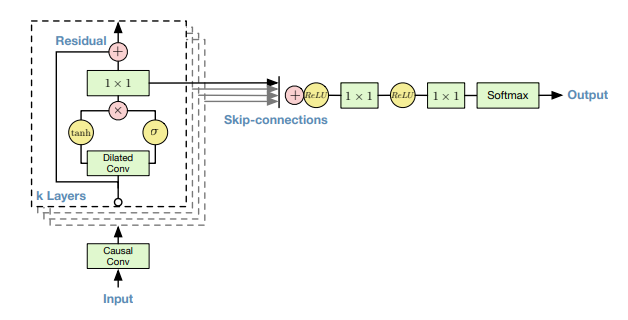
\includegraphics[width=5.5in]{images/DCCN_Layer.png}
    \caption{The structure of WaveNet's architecture.}
    \label{fig:dccnlayer}
\end{figure}

\begin{minted}{python}
import torch
from torch import nn

class DilatedCausalConv(nn.Module):
    def __init__(self, channels, dilation=1):
        super(DilatedCausalConv, self).__init__()

        self.conv = nn.Conv1d(channels, channels,
                            kernel_size = 2, stride=1,
                            dilation=dilation,
                            padding=0,
                            bias=False)

    def forward(self, x):
        output = self.conv(x)
        return output
\end{minted}

Next we will take on the more complicated task of defining our residual blocks. At this point, our implementation will diverge from the original paper. Rather than having one convolutional layer that outputs to both the residual and skip connections, each will get their own independently parameterized convolutional layer to allow for greater control in training. With this in mind, our residual block has five parts: A dilated convolution layer, $\tanh$ filter and sigmoid gate nonlinearities, an two $1\times1$ convolutional layers for the residual and skip connections. 

\begin{minted}{python}
class ResidualBlock(nn.Module):
    def __init__(self, residual_channels, skip_channels, dilation):
        super(ResidualBlock, self).__init__()

        self.dilated = DilatedCausalConv(residual_channels, dilation=dilation)
        self.residual_conv = nn.Conv1d(residual_channels, residual_channels, 1)
        self.skip_conv = nn.Conv1d(residual_channels, skip_channels, 1)

        self.filter_tanh = nn.Tanh()
        self.gate_sig = nn.Sigmoid()

\end{minted}
\newpage
\begin{minted}{python}

    def forward(self, x, skip_size):
        output = self.dilated(x)
        # Activated hidden state:
        filter = self.filter_tanh(output)
        gate = self.gate_sig(output)
        activated = gate * filter
        # Calculate the residual connection
        output = self.residual_conv(activated)
        cut_input = x[:, :, -output.shape[2]:]
        output += cut_input
        #Calculate and cut the skip connection to size
        skip = self.skip_conv(activated)
        skip = skip[:, :, -skip_size:]

        return output, skip
\end{minted}


At the forward pass after running our activated hidden state through the residual convolution, we cut the input to the length of the output and add. After running our hidden state through the skip convolution, we cut to the desired output size. Now that we have a definition for a single block, we can create a class that stacks them for modularity. At initialization, our residual stack class takes in the number of blocks and the number of layers per block, and at the forward pass, it recursively defines the input to the next model and keeps track of the skip connections before stacking them at the return.

\begin{minted}{python}
class BlockStack(nn.Module):
    def __init__(self, layer_size, stack_size, residual_channels, skip_channels):
        super(BlockStack, self).__init__()

        self.layer_size = layer_size
        self.stack_size = stack_size

        self.blocks = self.stack_blocks(residual_channels, skip_channels)

    def _dilations(self):
        dilations = []
        for stack in range(0, self.stack_size):
            for layer in range(0, self.layer_size):
                dilations.append(2 ** layer)
        return dilations

    def stack_blocks(self, residual_channels, skip_channels):
        return [ResidualBlock(residual_channels, skip_channels, d) for d in self._dilations()]

    def forward(self, x, skip_size):
        output = x
        skips = []
        for i in range(len(self.blocks)):
            block = self.blocks[i]
            output, skip = block(output, skip_size)
            skips.append(skip)
        return torch.stack(skips)
\end{minted}

Finally, we define the input and output networks. The input network is a simple $2\times1$ convolution with one sample worth of padding on either end. At forward, we clip off the last value to assure the input and output of this network are the same size. The purpose of this network is to get the input data up to the required number of channels to be put into the residual block. 

\begin{minted}{python}
class CausalConv(nn.Module):
    def __init__(self, in_channels, out_channels):
        super(CausalConv, self).__init__()
        self.conv = nn.Conv1d(in_channels, out_channels,
                            kernel_size=2, stride=1, padding=1,
                            bias=False)

    def forward(self, x):
        output = self.conv(x)
        return output[:, :, :-1]
        


class OutNet(nn.Module):
    def __init__(self, channels):
        super(OutNet, self).__init__()
        self.relu = nn.ReLU()
        self.layer1 = nn.Conv1d(channels, channels, 1)
        self.layer2 = nn.Conv1d(channels, channels, 1)
        self.sm = nn.Softmax(dim=1)

    def forward(self, x):
        output = self.relu(x)
        output = self.layer1(x)
        output = self.relu(x)
        output = self.layer2(x)
        return output
\end{minted}

Symmetrically, the purpose of the output network is to condense the stack of skip connections back down to the number of input channels. The output network uses two independent $1\times1$ convolutional layers each proceeded by a ReLU activation. The paper specifies that after the second convolution, the output should go through a softmax. However, we will be training using PyTorch's Cross Entropy Loss, which starts by calculating a softmax for us, so we can skip that step here.